%!TEX program = xelatex
\documentclass[UTF8]{ctexart}
    \usepackage{amsmath}
    \usepackage{geometry}
	\usepackage{graphicx}
	\usepackage[utf8]{inputenc}
	\usepackage{listings}
	\usepackage{url}
    \usepackage{verbatim}
	
	\graphicspath{ {./images/} }

    \title{第$6$章$6.11$编程实验 }
    \author{2016211305班 \ 熊光正 (学号:2016211249)}
\begin{document}
\lstset{numbers=left,frame=single,breaklines=true}
\maketitle
\section{实验环境}
本实验使用$Visual \ Studio \ Code$编辑器,在基于$x86\_64$指令集的$64$位中文$Windows \ 10$环境下开发。
程序使用$Clang$(版本号:$7.0.0$)编译器,基于$MSVC$环境进行编译,编译目标为$x86\_64-pc-windows-msvc$。
\section{程序1}
\subsection{源代码}
\begin{lstlisting}[language={C}]
// 1.c
typedef int A[10][20];
A a;
A *fun(){
    return (a);
}
int main(){
    fun();
}
    \end{lstlisting}
\subsection{编译输出}
\begin{lstlisting}
> clang 1.c -o 1.exe
1.c:5:12: warning: incompatible pointer types returning 'A' (aka 'int [10][20]') from a function with result type 'A *' (aka 'int (*)[10][20]'); take the address with &
        [-Wincompatible-pointer-types]
    return (a);
            ^~~
            &
1 warning generated.
    \end{lstlisting}
\subsection{结果截图}
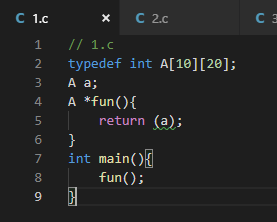
\includegraphics{1-code} \\
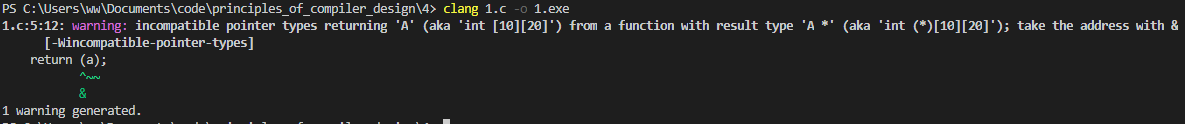
\includegraphics[width=\textwidth]{1-output}
\subsection{结果分析}
函数$fun$应返回$A*$,但语句$return (a)$返回了$A$,即
$$pointer(int[20]) \neq pointer(int[10][20]) = pointer(A)$$
,故编译器建议取其地址(take the address with \&)。
\section{程序2}
\subsection{源代码}
\begin{lstlisting}[language={C}]
// 2.c
typedef int A[10][20];
A a;
A *fun(){
    return (&a);
}
int main(){
    fun();
}
    \end{lstlisting}
\subsection{编译输出}
\begin{lstlisting}
(空)
    \end{lstlisting}
\subsection{结果截图}
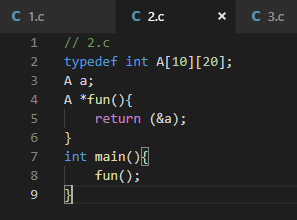
\includegraphics{2-code} \\
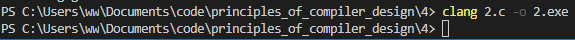
\includegraphics[width=\textwidth]{2-output}
\subsection{结果分析}
函数$fun$应返回$A*$,语句$return (\&a)$返回了$A*$,是合法的$A*$指针类型,故不出现错误或警告。
\section{程序3}
\subsection{源代码}
\begin{lstlisting}[language={C}]
// 3.c
typedef int A[10][20];
typedef int B[20];
A a;
B *fun(){
    return (a);
}
int main(){
    fun();
}
    \end{lstlisting}
\subsection{编译输出}
\begin{lstlisting}
    (空)
    \end{lstlisting}
\subsection{结果截图}
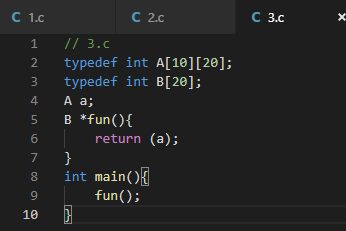
\includegraphics{3-code} \\
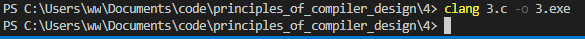
\includegraphics[width=\textwidth]{3-output}
\subsection{结果分析}
函数$fun$应返回$B*$,语句$return (a)$返回了$A$,即
$$pointer(int[20]) = pointer(B) = pointer(int[20])$$
,是合法的$B*$指针类型,故不出现错误或警告。
\section{程序4}
\subsection{源代码}
\begin{lstlisting}[language={C}]
// 4.c
#include <stdio.h>

typedef int A[10][20];
A a;
void fun(){
    printf("%d,%d,%d\n",a,a+1,&a+1);
}
int main(){
    fun();
}
    \end{lstlisting}
\subsection{编译输出}
\begin{lstlisting}
> clang 4.c -o 4.exe
4.c:7:25: warning: format specifies type 'int' but the argument has type 'int (*)[20]' [-Wformat]
    printf("%d,%d,%d\n",a,a+1,&a+1);
            ~~          ^
4.c:7:27: warning: format specifies type 'int' but the argument has type 'int (*)[20]' [-Wformat]
    printf("%d,%d,%d\n",a,a+1,&a+1);
               ~~         ^~~
4.c:7:31: warning: format specifies type 'int' but the argument has type 'A *' (aka 'int (*)[10][20]') [-Wformat]
    printf("%d,%d,%d\n",a,a+1,&a+1);
                  ~~          ^~~~
3 warnings generated.
    \end{lstlisting}
\subsection{结果截图}
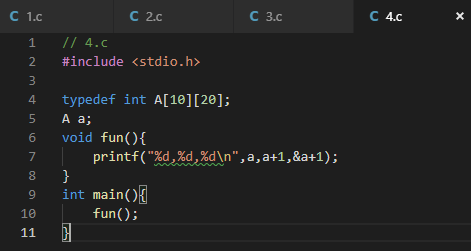
\includegraphics{4-code} \\
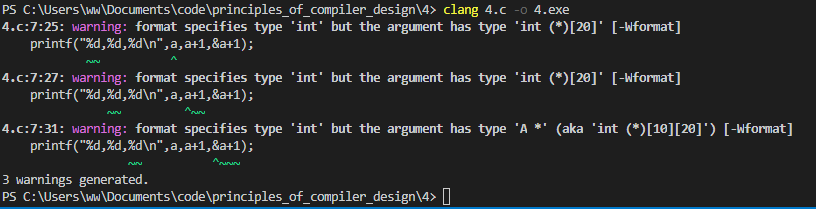
\includegraphics[width=\textwidth]{4-output}
\subsection{结果分析}
函数$fun$中,语句$printf("\%d,\%d,\%d \backslash n",a,a+1,\&a+1)$,$printf$函数希望输入$3$个$int$,
而程序输入$pointer(int[20])$、$pointer(int[20])$、$pointer(A)$,故出现警告。
\end{document}
